%! TEX program = pdflatex
%% Mauricio Caceres Bravo <mauricio.caceres.bravo@gmail.com>

%----------------------------------------------------------------------
\documentclass{article}

\usepackage[summary]{brownpreamble}
\usepackage{etoc}
\setcounter{tocdepth}{3}

\renewcommand{\subsectionmark}[1]{\markboth{#1}{}}
\renewcommand\sectiontype{Lecture \thesection:\ }
\lhead{\color{light-gray} \itshape Math Camp Aug 23, 2021 -- Lecture \thesection}
\rhead{\color{light-gray} \itshape \thesubsection. \leftmark}
\setcounter{section}{4}
% \renewcommand\SetHideLevel{1pt}

%----------------------------------------------------------------------
\begin{document}
\displayoptions

% \pgfplotsset{
%     compat=1.8,
%     every axis/.append style={
%         ,axis lines=center
%         ,xlabel style={anchor=south west}
%         ,ylabel style={anchor=south west}
%         ,zlabel style={anchor=south west}
%         ,tick align=outside
%     },
% }

\begin{figure}[H]
  \centering
  \caption{Graphical Illustration of the Envelope Theorem Ctd.}
  \label{fig:graphical_illustration_of_the_envelope_theorem_ctd}
  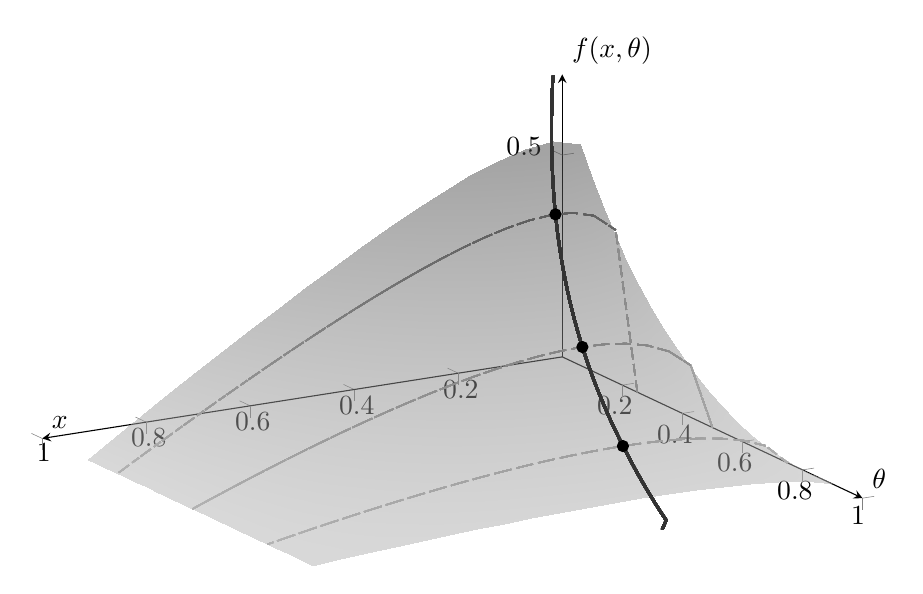
\begin{tikzpicture}
      \begin{axis}[name=plot1
        ,view={150}{30}
        ,width=12cm
        ,height=8cm
        ,zmin=0
        ,zmax=0.7
        ,xmin=0
        ,xmax=1
        ,ymin=0
        ,ymax=1
        ,ylabel=$\theta$
        ,xlabel=$x$
        ,zlabel={$f(x, \theta)$}
        ,colormap={whiteblack}{color(0cm)  = (black!30); color(1cm) = (black)}
        ,axis lines=center
        ,xlabel style={anchor=south west}
        ,ylabel style={anchor=south west}
        ,zlabel style={anchor=south west}
        ,tick align=outside
      ]
      \addplot3 [
        surf
        ,shader=interp
        ,fill opacity=0.5
        ,samples=20
        ,domain=0:1
        ,y domain=0.15:0.9
        % ,on layer=foreground
      ] {x^y-x};
      \addplot3[
        variable=t
        ,samples=40
        ,mesh
        ,domain=0:1
        ,color=black!80
        ,line width=1pt
      ] ({t^(1/(1 - t))},t,{t^(t/(1 - t)) - t^(1/(1 - t))});
      \addplot3[variable=t, mesh, dashed, opacity=0.8, domain=0:1, line width=0.5pt, on layer=foreground] (t,0.25,{t^0.25 - t});
      \addplot3[variable=t, mesh, dashed, opacity=0.8, domain=0:1, line width=0.5pt, on layer=foreground] (t,0.5,{t^0.5 - t});
      \addplot3[variable=t, mesh, dashed, opacity=0.8, domain=0:1, line width=0.5pt, on layer=foreground] (t,0.75,{t^0.75 - t});
      \addplot3 [only marks, mark=*] coordinates {
        (0.1574901, 0.25, 0.4724704)
        (0.25,      0.5,  0.25)
        (0.3164062, 0.75, 0.1054688)
      };
      \end{axis}
  \end{tikzpicture}
\end{figure}

% ---------------------------------------------------------------------
\end{document}

